\documentclass[../main.tex]{article}

\begin{document}

\section{Introduction}

The southern live oak (\textit{Quercus virginiana}) lives in the southeastern US (\textcite{Cavender-Bares2015}, Figure ~\ref{fig:map}).

\begin{figure}[ht!]
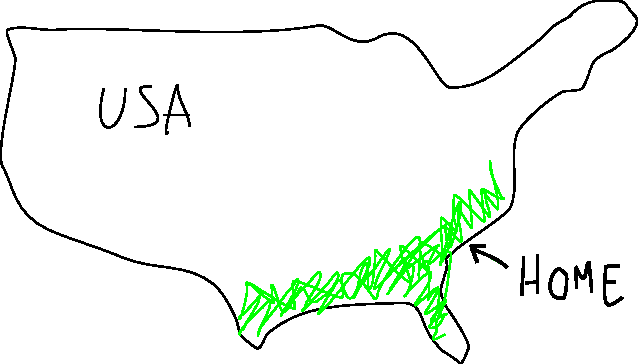
\includegraphics[width=0.4\textwidth]{map.pdf}
\centering	
\caption{Southern live oak's home.}
\label{fig:map}
\end{figure}

It likes to do photosynthesis and produce acorns. It is said that their acorns germinate better after being eaten and pooped by gators \parencite{CavenderBares2027}. Is this really true?

\end{document}
